\chapter{Progressions}

Figure~\ref{iiprog} presents one of the most common truisms circulated regarding jazz harmony in a new form.  Each of the curves plotted here describes the statistical behavior of a chord category following the appearance of a locally-transposed $ii$ chord.\footnote{For details regarding the key-finding and local transposition, see Chapter 2.}  The details of Figure~\ref{iiprog} will emerge below, but the general form of the plot is simple: the vertical axis gives a measure of probability, while the horizontal displays time elapsed after a $ii$ chord.  Each curve tracks the probability of a particular chord appearing after $ii$ over time.

\begin{figure}
	\centering
	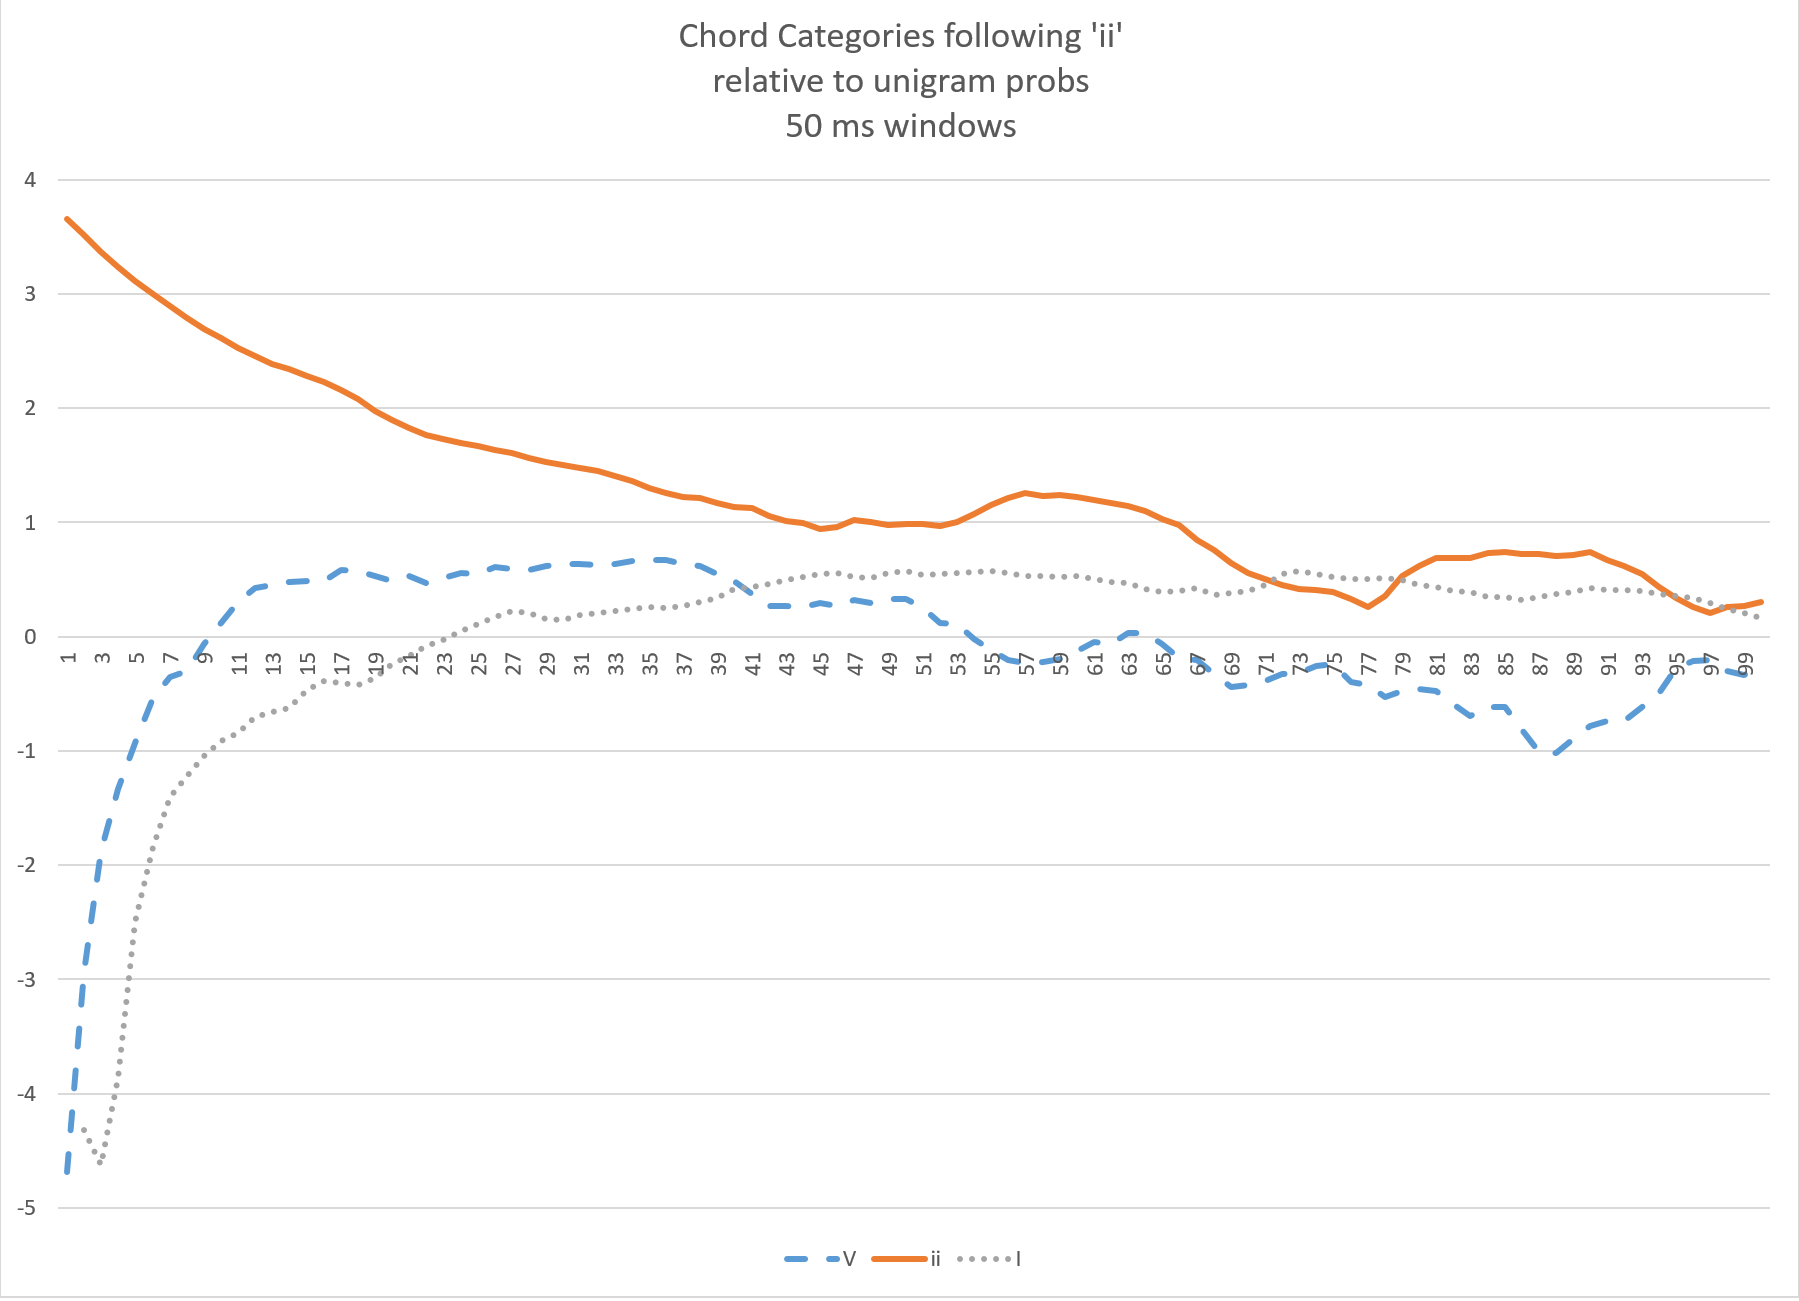
\includegraphics[width=5.8in]{iiprogressions.png}
	\caption{The unigram-relative log probabilities of $ii$ (blue, dashed line), $V$ (gray, dotted line), and $I$ (red line) versus time (in milliseconds) elapsed after a $ii$ chord in the YJaMP corpus.  Here, the categories for $V$, $ii$, and $I$ have been hand-chosen; Chapter 4 provides a means to bootstrap category formation.}
	\label{iiprog}
\end{figure}

The truism: in jazz, $ii$ often progresses to $V$ and then to $I$.  The curves of Figure~\ref{iiprog} have different shapes -- different behaviors over time -- which might be said to demonstrate and destabilize the truism in and with explicitly temporal terms.  The (gray, dotted) curve for $V$ rises to a probability peak between 500 and 2000 milliseconds, after which it slowly decreases in probability.  The (red, solid) curve for $I$ starts out less probable than $V$, but it becomes more probable as time elapses, surpassing $V$ around 2000ms.  Cast in traditional terms, these curves imply that when a $ii$ chord appears, it is likely that a $V$ chord appears some short time later, while a $I$ chord will probably appear some time after that.  This representation avoids bigram-style transitions between immediately adjacent states, instead displaying probabilistic tendencies over time.

The (blue, dashed) curve corresponding to $ii$ on Figure~\ref{iiprog} seems superfluous with respect to the truism above.  It shows that at very short times after the appearance of a $ii$ chord, another (or perhaps the same) $ii$ chord is highly probable.  When compared to the other curves on the plot, the $ii$ curve shows a very different shape and behavior.  I will return to this and the details of Figure~\ref{iiprog} in the following sections, but for now it suffices to note that this plot encapsulates at least two different scales of behavior: local reappearance of $ii$ and ``delayed" (however minimally) appearance of $V$ and $I$.  These modes of progression place it into dialog with schematic diagrams like Figure~\ref{pers}, taken from the harmonic progression work of Christopher Wm. White and Ian Quinn.\footnote{See \cite{wq2017}.}

\begin{figure}
	\centering
	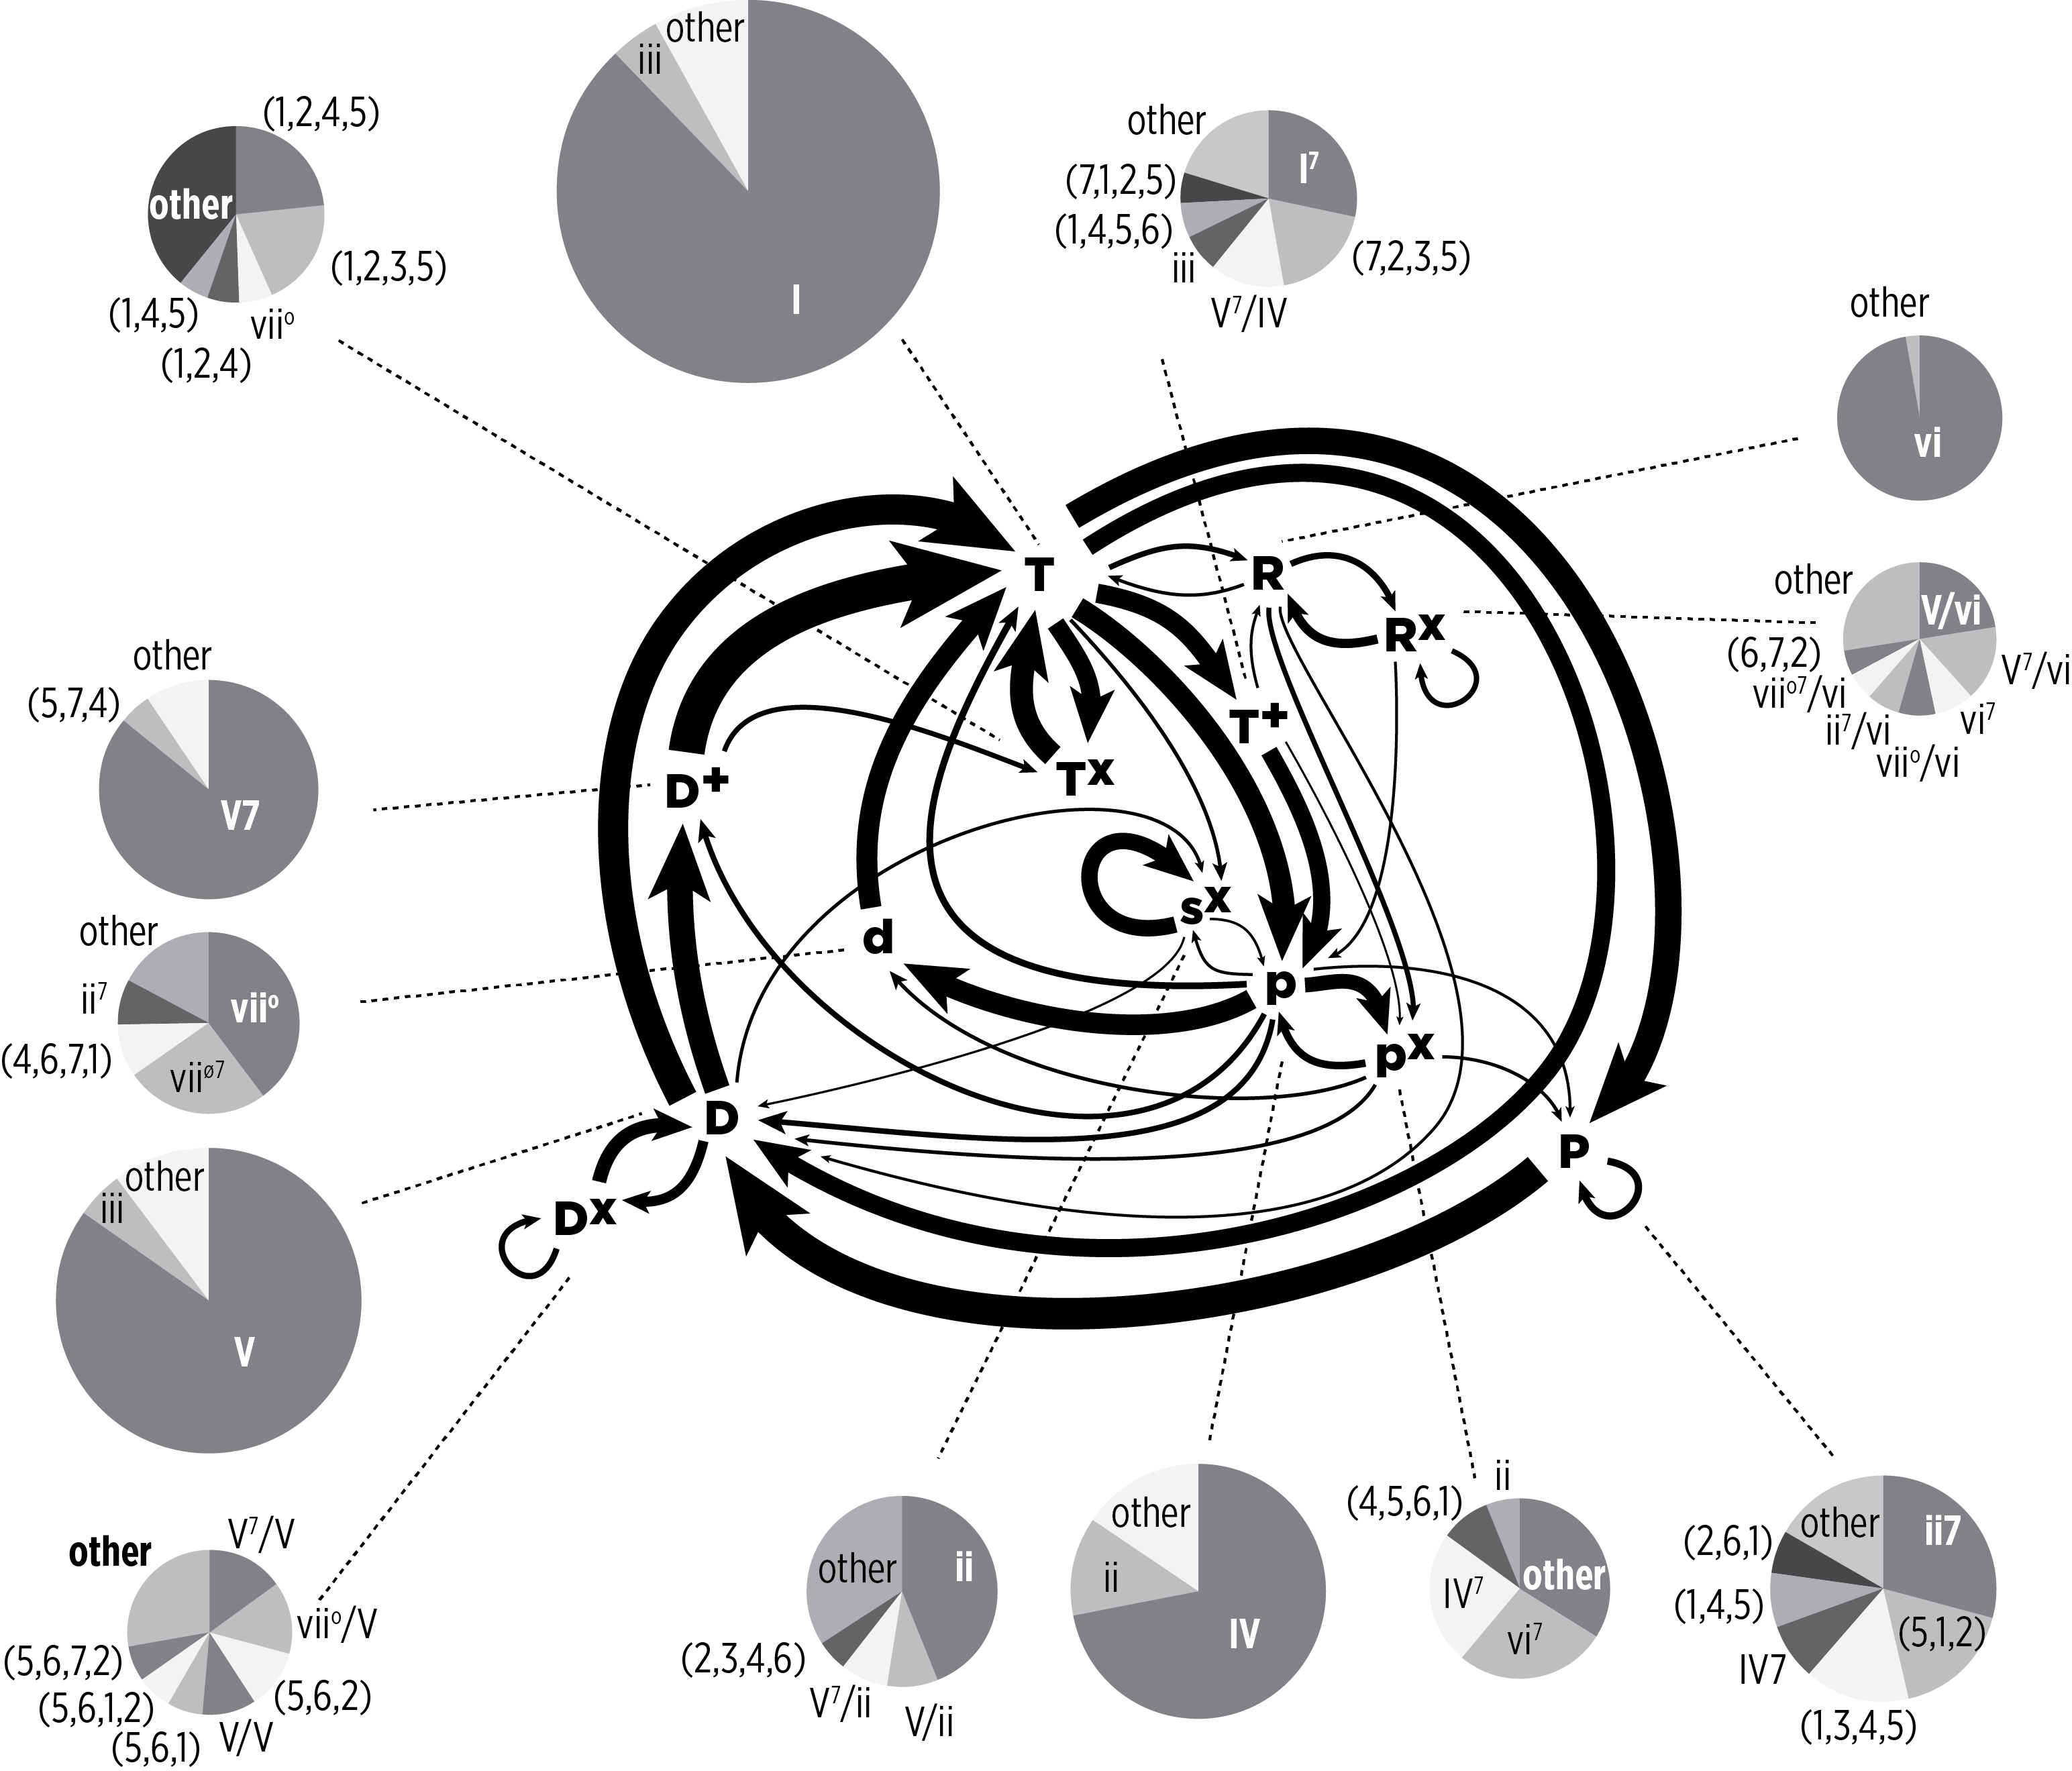
\includegraphics[width=5.5in]{WhiteQuinn_NewPersimmon.png}
	\caption{An empirically-derived ``persimmon" model of functional progression in the Bach chorales, taken from \cite{wq2017}.  Dotted lines indicate chord membership within functional categories.  Solid arrows indicate category-level progressions, whether function-preserving (self-progressions) or not (syntactic progressions).  While this diagram encodes progressions on different time scales, neither the progressions nor the functional categories engage with the temporal structure of the data.}
	\label{pers}
\end{figure}

On its most basic level, the ``persimmon" of Figure~\ref{pers} includes a combination of pitch-based chord labels (roman numerals) and functional categories ($T$, $S$, $D$, $P$, and $R$) linked by a variety of arrows.  For each functional category, the dotted lines on the figure provide a mapping indicating the kinds of chords likely to appear as members of the category.  Between categories themselves, solid arrows indicate common functional progressions.  Some progressions are from one syntactic function to another -- say, $T \rightarrow P$ or $P \rightarrow D$ -- while others indicate ``self-progressions" like $T \rightarrow T^x \rightarrow T$.  Each arrow thus corresponds to a chord transition, an immediately-adjacent bigram, and the actual pitch content of such a transition can be drawn from the pie-chart distributions relevant to each category.

Figure~\ref{iiprog} shows something similar to the solid, functional progression arrows on the persimmon, though it replaces the bigram orientation with a more explicit engagement with time.  While Figure~\ref{pers} indicates that $ii^7$ as predominant (P) frequently progresses to $V$ as dominant (D), Figure~\ref{iiprog} indicates temporal limits to such a claim; at very short and very long time scales, the $ii$ chords captured by Figure~\ref{iiprog} hardly progress to $V$ in any significant way, and it is only in a certain temporal regime that the $ii \rightarrow V$ syntactic progression claim seems to live.

This chapter provides a case study exposing the machinery behind and implications of Figure~\ref{iiprog} and its ability to describe multiple \emph{temporal progression regimes} within a single statistical framework.  Examples of short-timespan self-progressions (like the blue $ii$ curve) and moderate-timespan syntactic progressions (like the gray $V$ curve) motivate the automated extraction of chords to which $ii$ tends to ``progress" at different time scales.  Principal component analysis (PCA), a frequent tool in computational time series analysis, will aid in reducing the temporal complexity of the many possible chords succeeding $ii$ at many possible scales.  A consideration of the most common ways $ii$ chords progress in time will suggest the possibility of ``bootstrapping" our types of progression, unearthing different temporal progression regimes without analytical inputs and directly from the statistical properties of YJaMP's solo piano performances.\footnote{The use of ``bootstrap" here draws on a long computational tradition of responding to a clear problem: if programmatic algorithms generate or load outputs from a series of inputs, how can a system receive the initial impetus to get off the ground?  (For early use of the term in this manner, see \cite{buchholz1953}).  The software term ``booting" seems to draw on the computational prehistory of pulling oneself up by one's ``bootstraps.")  I hand-supply plausible chord categories here, but I intend this as an initial approximation to be modified subsequently by machine learning methods.}  The case study here serves to anchor chord progressions in a temporal framework amenable to computation, and its methods apply to any scale-degree set in the corpus.  As Chapter 4 will indicate, the resulting temporal representation both captures nuanced progression behavior for individual chords and permits the construction of syntactic categories via elementary machine learning.  In the Kockelmanian terms of Chapter 2, the algorithms of this chapter turn scale-degree set signed indices into interpretants well-suited to the algorithmic agents of Chapter 4.

\section{Chords and Time}
%Chord ``behavior" different on different time scales
%Smallest: static, mostly self-transitions, lends itself to phonetic models
%Small: local behavior, mostly voice-leading neighbors
%Middle: ``Syntactic" models apply, here; suppressions (V-IV) and correlations (V-I)
%Large: predictive power recedes to background statistics (X-...-I)

Temporality and probability lie at the heart of Figure~\ref{iiprog}'s presentation of harmonic progressions.  These two concepts are concretized by the introduction of particular harmonic objects.  In the previous section, the term ``chord category" (applied to $ii$, $V$, and $I$) reflects an artificial (but rather conventional) definition of $ii$ as a category which includes the locally-transposed scale-degree sets $[2,5,9]$, $[0,2,5,9]$, and $[0,2,5]$.\footnote{In conventional scale degree terms, these chords are $(\hat{2},\hat{4},\hat{6})$, $(\hat{1},\hat{2},\hat{4}, \hat{6})$, and $(\hat{1},\hat{2},\hat{4})$.  For further details on the production of YJaMP scale-degree sets, see Chapter 2.}  As seen in Chapter 2, these scale degree sets represent the three most common instantiations of western-classical $ii$ chords produced via algorithmic parsing of the YJaMP corpus.  Along similar lines, the $V$ and $I$ categories indicated on Figure~\ref{iiprog} contain ($[2,7,11]$, $[2,5,7,11]$, $[5,7,11]$) and ($[0,4,7]$, $[0,3,7]$, $[0,4,11]$, $[0,3,10]$, $[0,4,7,11]$, $[0,3,7,10]$), respectively.  Machine learning methods will replace these chord category assumptions in Chapter 4, but they appear here as the simplest way to connect functional category concepts from traditional harmony to computational time series analytical methods.

The horizontal axis of Figure~\ref{iiprog} represents time in milliseconds.  Strictly speaking, the plotted probabilities do not provide continuous data; instead, each 50-millisecond time window has been ``binned," where its contents are assumed to be simultaneous enough to warrant consideration as a potential chord in the way outlined at the end of Chapter 2.  The left hand side of the figure, where $t=0$, is the time at which a $ii$ chord appears; $t=500$ is 500ms later (one half second), and $t=5000$ is 5 seconds after the initial $ii$ chord.  Each point on a plotted curve indicates how much more or less likely the curve's chord is to be found $t$ milliseconds after a $ii$ chord than it is to be found in the corpus in general.  A Python algorithm finds every instance of a $ii$ chord in the YJaMP performances and tracks the time delay with which each chord appears in the subsequent 5 seconds.  A kind of composite statistical template results: given $ii$ as an ``origin chord," the algorithm returns a probability distribution for each subsequent 50ms window in which it accounts for every ``destination chord" found that long after a $ii$ chord.  These probability distributions consist of coded versions of claims like ``$t$ milliseconds after a $ii$ chord, chord $x$ appears $y$ orders of magnitude more often than it does in the corpus generally."  

This claim does not reference the absolute probability of appearance for the ``destination" chord $x$ directly, since such a statistic would not make plain the predictive or syntactic importance of $ii$ itself.  A chord highly probable (in absolute terms) at some time $t$ might reflect a high background \emph{unigram} probability independent of the nearby presence of $ii$.\footnote{For further details on the quasi-Zipfian unigram distribution of the YJaMP corpus, see Chapter 2.}  Figure~\ref{iiprog} normalizes these distributions, however, plotting the difference between two logarithmic probabilities on the vertical axis:
\begin{equation}
P(x,t) = \log_{10} \big( p(x\mid ii,t) \big) - \log_{10} \big( p(x) \big)
\end{equation}
Here, $P(x,t)$ is the relative log probability of chord $x$ at time $t$ plotted on the vertical axis of Figure~\ref{iiprog}, while $p(x)$ and $p(x\mid ii,t)$ are the probabilities of $x$ in the corpus at large and given the previous occurrence of $ii$ $t$ milliseconds previously, respectively.  Subtracting these logarithmic probabilities performs a normalization similar to dividing the (non-log) probability-given-$ii$ by the probability-in-general.  The result of the logarithmic normalization is that the positive vertical axis values of Figure~\ref{iiprog} indicate probabilities higher than the background unigram distribution, while negative axis values indicate that the given chord occurs less frequently at a given delay $t$ after $ii$ than it does in the corpus in general -- that the chord is suppressed by $ii$.  Each increase of one unit on the vertical axis corresponds to a particular chord occurring 10 times more probably at a given time $t$ than its unigram probability.

%talk about using these curves as templates for isolating types of progression behavior into different temporal regimes.
If the curves of Figure~\ref{iiprog} show the relative probabilities of three destination chords, they stand as a way of quantifying the effect of the origin chord ($ii$) on the presence of subsequent -- and not necessarily adjacent -- $ii$, $V$, and $I$ chords.  The appearance of $ii$ has one particular kind of effect at short distances: it makes other $ii$ chords much more probable.  But how many chords does $ii$ impact in a similar way, and how many kinds of effect does $ii$ have?

\begin{figure}
	\centering
	\caption{An excerpt of the temporal probability distributions for common chords following $ii$ (unigram-relative log probabilities versus time).  Traditional harmonic theory assumes the ability to reduce this complex temporal data to time-independent category transition rules.}
	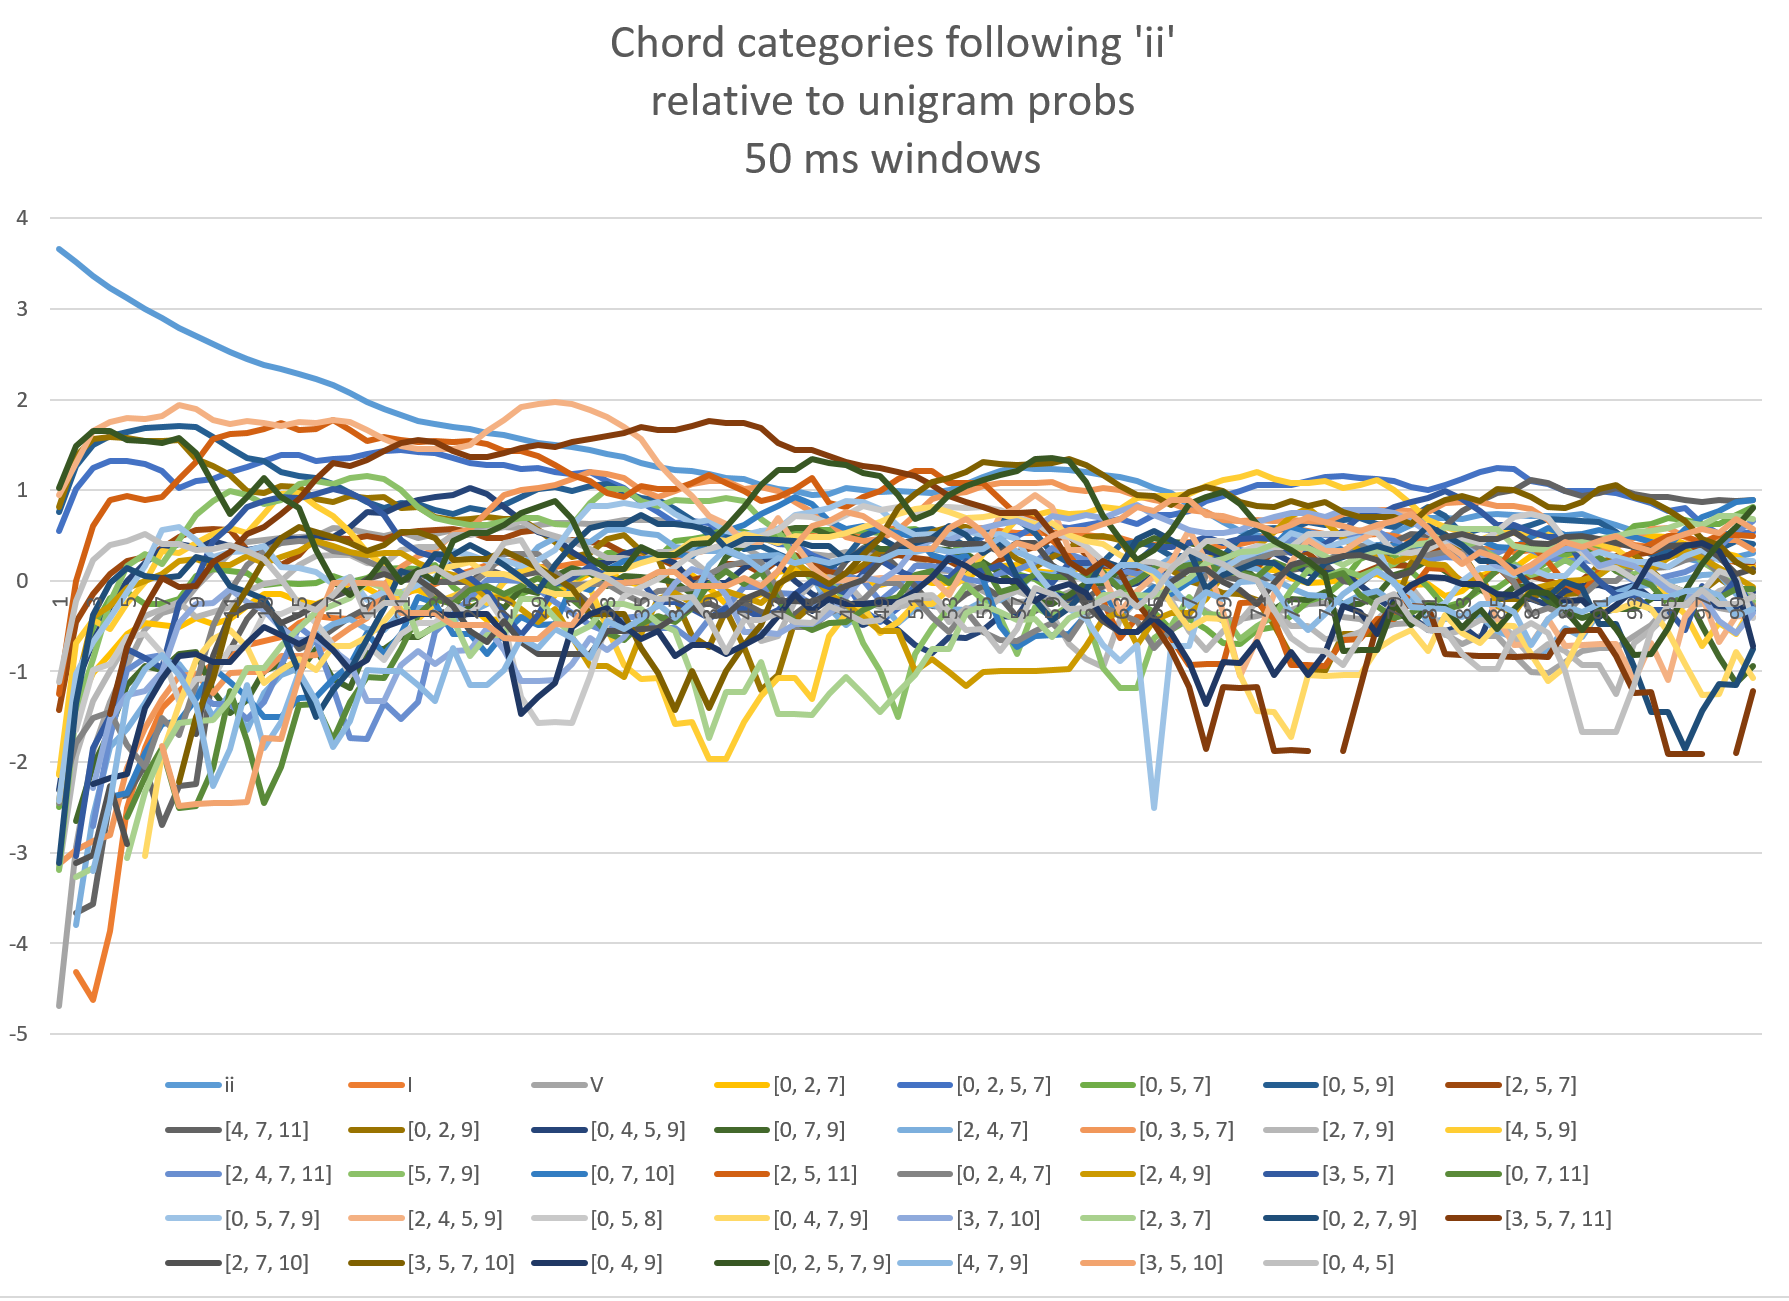
\includegraphics[width=6in]{ii_messy.png}
	\label{ii_messy}
\end{figure}

Figure~\ref{ii_messy} presents a small fraction of the destination chord probability distributions for chords following $ii$.  For many high-probability origin chord types in the corpus (like $ii$), tokens corresponding to more than 1000 distinct destination chord types appear within the 5 seconds following all of the origin chord's tokens across the corpus.  Sorting through these distributions by hand is not feasible, and many of the destination chords are low-probability objects in the first place; there is no guarantee that random fluctuations in the appearance of rare chords will tell us anything about $ii$'s syntactic properties.

But to find other chords strongly impacted by $ii$ in ways similar to the behavior displayed in Figure~\ref{iiprog}, it suffices to compare the large number of destination chord probability distributions to the (blue, gray, and red) templates provided by $ii$, $V$, and $I$.  Curves which lie close to the $V$ curve correspond to chords with temporal behavior similar to $V$ in the context of $ii$.  This sounds tautological, but an important distinction is at play: a chord with a temporal probability distribution similar to that of $V$ on Figure~\ref{iiprog} may have absolutely no discernible pitch relation to $V$ as a scale-degree set.  ``$V$-like" chords, distributionally speaking, need only \emph{act like} $V$, statistically, in the temporal context of $ii$.  In other words, an algorithmic agent calculating which destination chord probability distributions from Figure~\ref{ii_messy} lie closest to those shown in Figure~\ref{iiprog} picks out chords which display temporal behavior similar to self-progressions ($ii \rightarrow ii$), syntactic progressions $(ii \rightarrow V$), and key-appropriate non-syntactic progressions ($ii \rightarrow I$).  This readily automatable process can assemble chord progression categories on more than one time scale -- and it can be performed for any origin chord.

\section{Phonetic scale}
On the shortest of musical time scales, the $ii$ chord tends to predict itself quite strongly, and it does so with diminishing strength as time passes.  To find what other chords behave this way after the appearance of $ii$, a few lines of code iterate across all of the observed destination chord distributions.  For each destination chord $d$, the code sees an $n$-dimensional probability vector, where $n$ can range up to the value of $t/50$ corresponding to the maximum windowed time delay for which statistics are kept.  It compares this vector to the $n$-dimensional ``self-progression" prototype (the $ii \rightarrow ii$ distribution) element-wise, subtracting the log probability of the current destination chord ($p_d$) from the log probability of the $ii$ chord ($p_{ii}$) at each time window.  Summing the absolute value of all of these deviations gives a simple metric for how dissimilar the destination chord is from $ii$:
\begin{eqnarray}
p_{ii} &=& (x_1, x_2, ... ,  x_n) \nonumber \\
p_{d} &=& (y_1, y_2, ..., y_n) \nonumber \\
D_{(ii,d)} &=& \sum_{i=1}^{n} \lvert y_i - x_i \rvert
\end{eqnarray}
That is, the code subtracts the probability of the origin chord $ii$ in window 1 (0-50ms) from the probability of the destination chord $d$ in window 1, takes the absolute value of the difference, and combines the resulting distances over $n$ consecutive time windows.  Setting $n$ is a matter of taste; I have chosen here to compare curves out to where the behavior of the prototype begins to level off.\footnote{As I will discuss below, PCA serves to diminish the importance of any particular choice of $n$, though it is important to track temporal statistics far enough to capture syntactic behavior.}  Minimizing the dissimilarity $D_{ii,d}$ given by Equation (3.1) provides a list of the destination chords which best fit the short-term behavior of $ii$.  A plot of the 5 best destination chords of this type is given in Figure~\ref{ii_phonetic}.

\begin{figure}
	\centering
	\caption{The 5 destination chords for $ii$ progressions with temporal probability distributions most similar to that of $ii \rightarrow ii$ (unigram-relative log probabilities versus time).}
	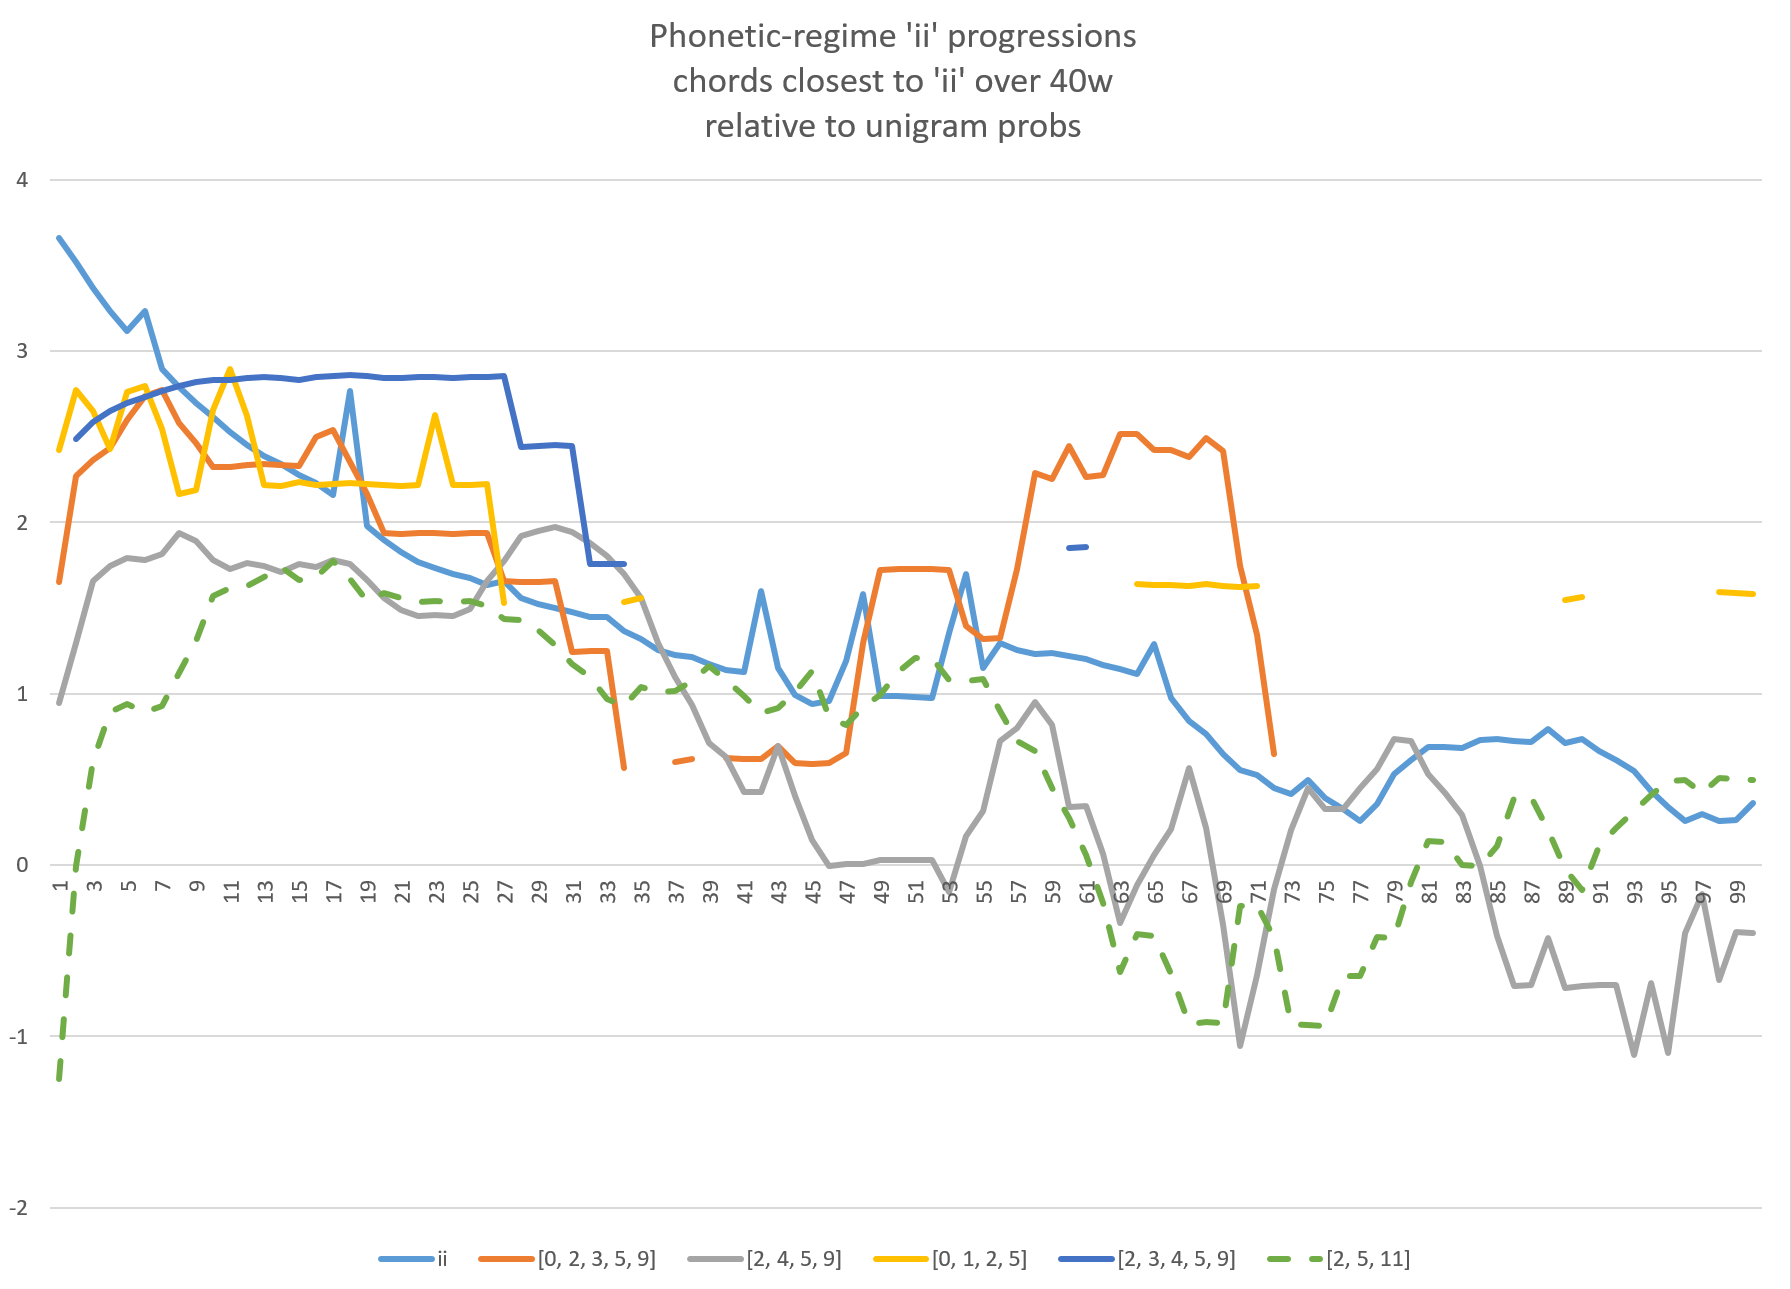
\includegraphics[width=6in]{ii_phonetic.png}
	\label{ii_phonetic}
\end{figure}

The results are striking in their predictability.  While pitch class/scale degree content played no role in the selection of self-progression destinations for $ii$, most of the destination chords with behavior most similar to $ii$ consist of some form of $ii$ chord with one or more added tones. $[0,2,3,5,9]$ and $[2,4,5,9]$ likely draw scale tones from their minor and major tonics, respectively, while $[0,1,2,5]$ and $[2,3,4,5,9]$ appear to arise from some local melodic motion.  In general, the list of self-progression partners for $ii$ suggests two rough categories of behavior:
\begin{enumerate}
	\item The destination chord may be related to the origin $ii$ chord by harmonic or quality completion.  Example: $[0,2,5] \rightarrow [0,2,5,9]$.
	\item The destination chord may be related to the origin $ii$ chord by the introduction of melodic notes. Example: $[0,2,5,9] \rightarrow [0,2,3,5,9]$.
\end{enumerate}
The two types of behavior can be combined, and there are also conditions where a self-progression may ambiguously result from either (i.e., $[2,5,9] \rightarrow [0,2,5,9]$).  In traditional music theory parlance, identifying chord ``progressions" in this context provides an alternate grounding for voice-leading or prolongational reduction rules.

In general, few of the progressions at this time scale consist of transitions which an analyst would deem sufficient to indicate a change of ``chord" or ``function."  Moreover, several self-progressions consecutively might be necessary to fill out all the pitches implied by an analyst's roman numeral.  As a result, I refer to this temporal progression time scale as the \emph{phonetic regime}, by way of analogy to linguistics.  In the way that multiple phonemes might make up a word, multiple self-progressions in this regime might make up a functional chord, and the particular ways in which phonetic regime chords are connected to one another rely on particular choices of voicing and melodic context in much the same way that the surface-level phonetic traces of linguistic syntax depend on the particulars of word order and nearby syntactic partners.  If harmonic syntax is to include primarily progressions from one function to another, then the phonetic regime provides a clean and empirically-grounded sense of the morphological transformations necessitated by concatenating syntactic partners. 

So far, I have avoided mentioning the fifth most $ii$-like member of the phonetic progression regime, shown in Figure~\ref{ii_phonetic}: $[2,5,11]$.  This chord, usually labeled $vii^{\circ}$, is not typically said to have the same function as $ii$.  Its presence on the plot might imply two things: that $[2,5,11]$ may appear as a phonetic neighbor to a more normative $ii$ chord (like $[2,5,9]$), or that destination chord curves this far below the self-progression $ii \rightarrow ii$ prototype begin to behave more like syntactic progression destinations than phonetic ones.  The $[2,5,11]$ distribution of Figure~\ref{ii_phonetic} falls almost exactly midway between the prototype curves for $ii$ and $V$ on Figure~\ref{iiprog}, and its behavior in different contexts might suggest assigning it a dual status, playing a role in the phonetic and syntactic regimes.  I mean the progression regime assignments to be fuzzy, in that limiting cases may exhibit behavior ill-captured by a single regime.

Chord category formation -- the set of decisions regarding what chords should make up a functional, syntactic category -- involves much more than a quick perusal of Figure~\ref{ii_phonetic}.  Comparing destination chord regimes across many (non-$ii$) origin chords provides a much broader data set well-suited to machine learning techniques, the results of which appear in Chapter 4.  To complete the $ii$ temporal progression case study, I turn here to another important time scale implied by Figure~\ref{iiprog}.

\section{Local syntactic scale}
Finding syntactic progressions amounts to a change in time scale.  The previous section showed that self-progression destination chords could be found by calculating which distributions most closely resembled that of $ii\rightarrow ii$ over short time scales, regardless of pitch content.  The same logic applies to functional syntactic progressions: if $ii\rightarrow V$ is a prototypical syntactic progression, destination chords at the time scale of the ``syntactic regime" should have temporal probability distributions similar to that of $V$ over moderate time scales.  Judging from Figure~\ref{iiprog}, the time scale relevant to that behavior stretches out to about 3 seconds.\footnote{Here, again, I describe the time scale cutoff intuitively, assuming that the initial suppression, sharp increase in probability, and return to unigram probability are all features of syntactic-$V$-ness.  It is unclear, in this description, if the lower-probability fluctuations at the end of the temporal tail bear important information; PCA will treat this problem below.}  Comparing all the destination chord probability distributions to $ii \rightarrow V$ over the time domain $(0,3000ms)$, we can again extract those most similar.  The seven best-fitting curves appear in Figure~\ref{ii_syntactic}.

\begin{figure}
	\caption{The 7 destination chords following $ii$ with syntactic regime probability distributions most closely resembling that of $ii \rightarrow V$.  Chords resembling both $V$ (solid curves) and $IV$ (dotted curves) appear to behave similarly.}
	\label{ii_syntactic}
	\centering
	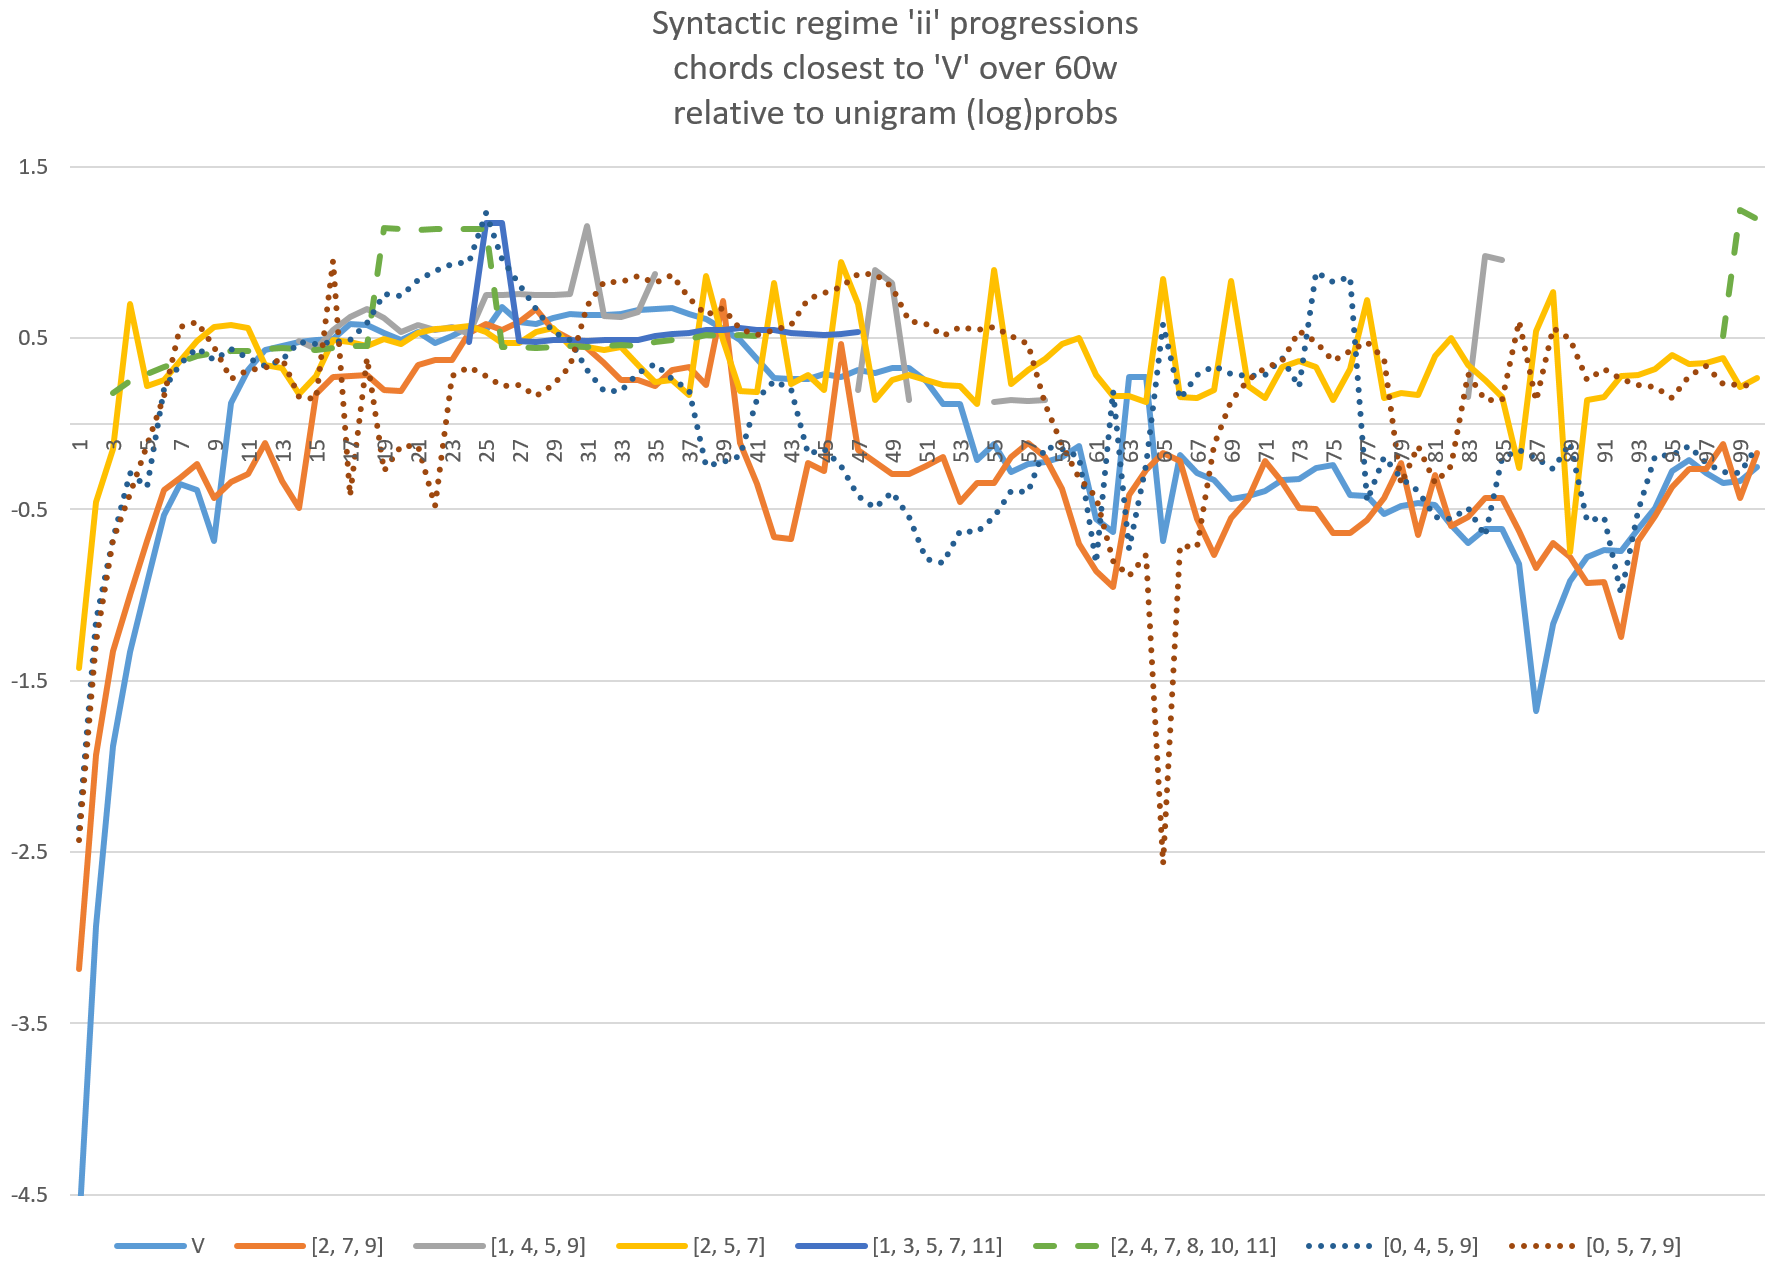
\includegraphics[width=6in]{ii_syntactic.png}
\end{figure}

Many of the destination chords which most closely mimic $V$ in this context are chords we might think of as phonetically-related to $V$ proper (see the solid curves on Figure~\ref{ii_syntactic}).  $[1,3,5,7,11]$ can be parsed as a $V^{\sharp 11 \flat 13}$, and $[2,5,7]$ may function as an incomplete $V^7$.  $[2,7,9]$ might be related to $[2,7,11]$ by melodic step, or it could be a symptom of more complicated behavior in play; $[2,4,7,8,10,11]$ is almost certainly the latter, and I have drawn it with dashes to indicate its ambiguous traditional interpretation.  But the syntactic nature of the $ii \rightarrow V$ curve does more than pick out the phonetic neighbors of $V$.  Since the temporal similarity metric assumes no pitch class or root similarities whatsoever, behavioral similarity also strongly selects another type of chord likely to follow $ii$: $IV$ chords.  Shown in the dotted curves of Figure~\ref{ii_syntactic}, $[0,4,5,9]$ and $[0,5,7,9]$ are both likely to follow $ii$ in a way similar to $V$ -- both types of chord would be deemed syntactic if found a moderate time after $ii$.

In this way, syntactic regime progression data partly reproduces and partly cuts across traditional functional harmony expectations.  Crucially, not all chords which behave like $V$ after $ii$ will \emph{always} behave like $V$; in other origin chord contexts, their behavior might be highly differentiated.  Each possible origin chord provides a distinct set of phonetic and syntactic data which might be used for functional categorization.  The $ii$ syntactic data here indicates a category of ``chords which follow $ii$ at moderate delays," of which both $IV$ and $V$ are members, but other syntactic data might distinguish the two.  In the context of $V$ origin chords, for example, the two fall into generally distinct regimes.  As Figure~\ref{V_phonetic} indicates, $V \rightarrow V$ is a phonetic-type progression, and in this regime, no chords resembling $IV$ are probable.

\begin{figure}[h]
	\caption{Phonetic regime self-progression destination chords following the appearance of $V$.  The pitch structure of these chords resembles that of $V^{(7)}$, but they appear here exclusively because their temporal statistics are most similar to those of $V \rightarrow V$ progressions.}
	\label{V_phonetic}
	\centering
	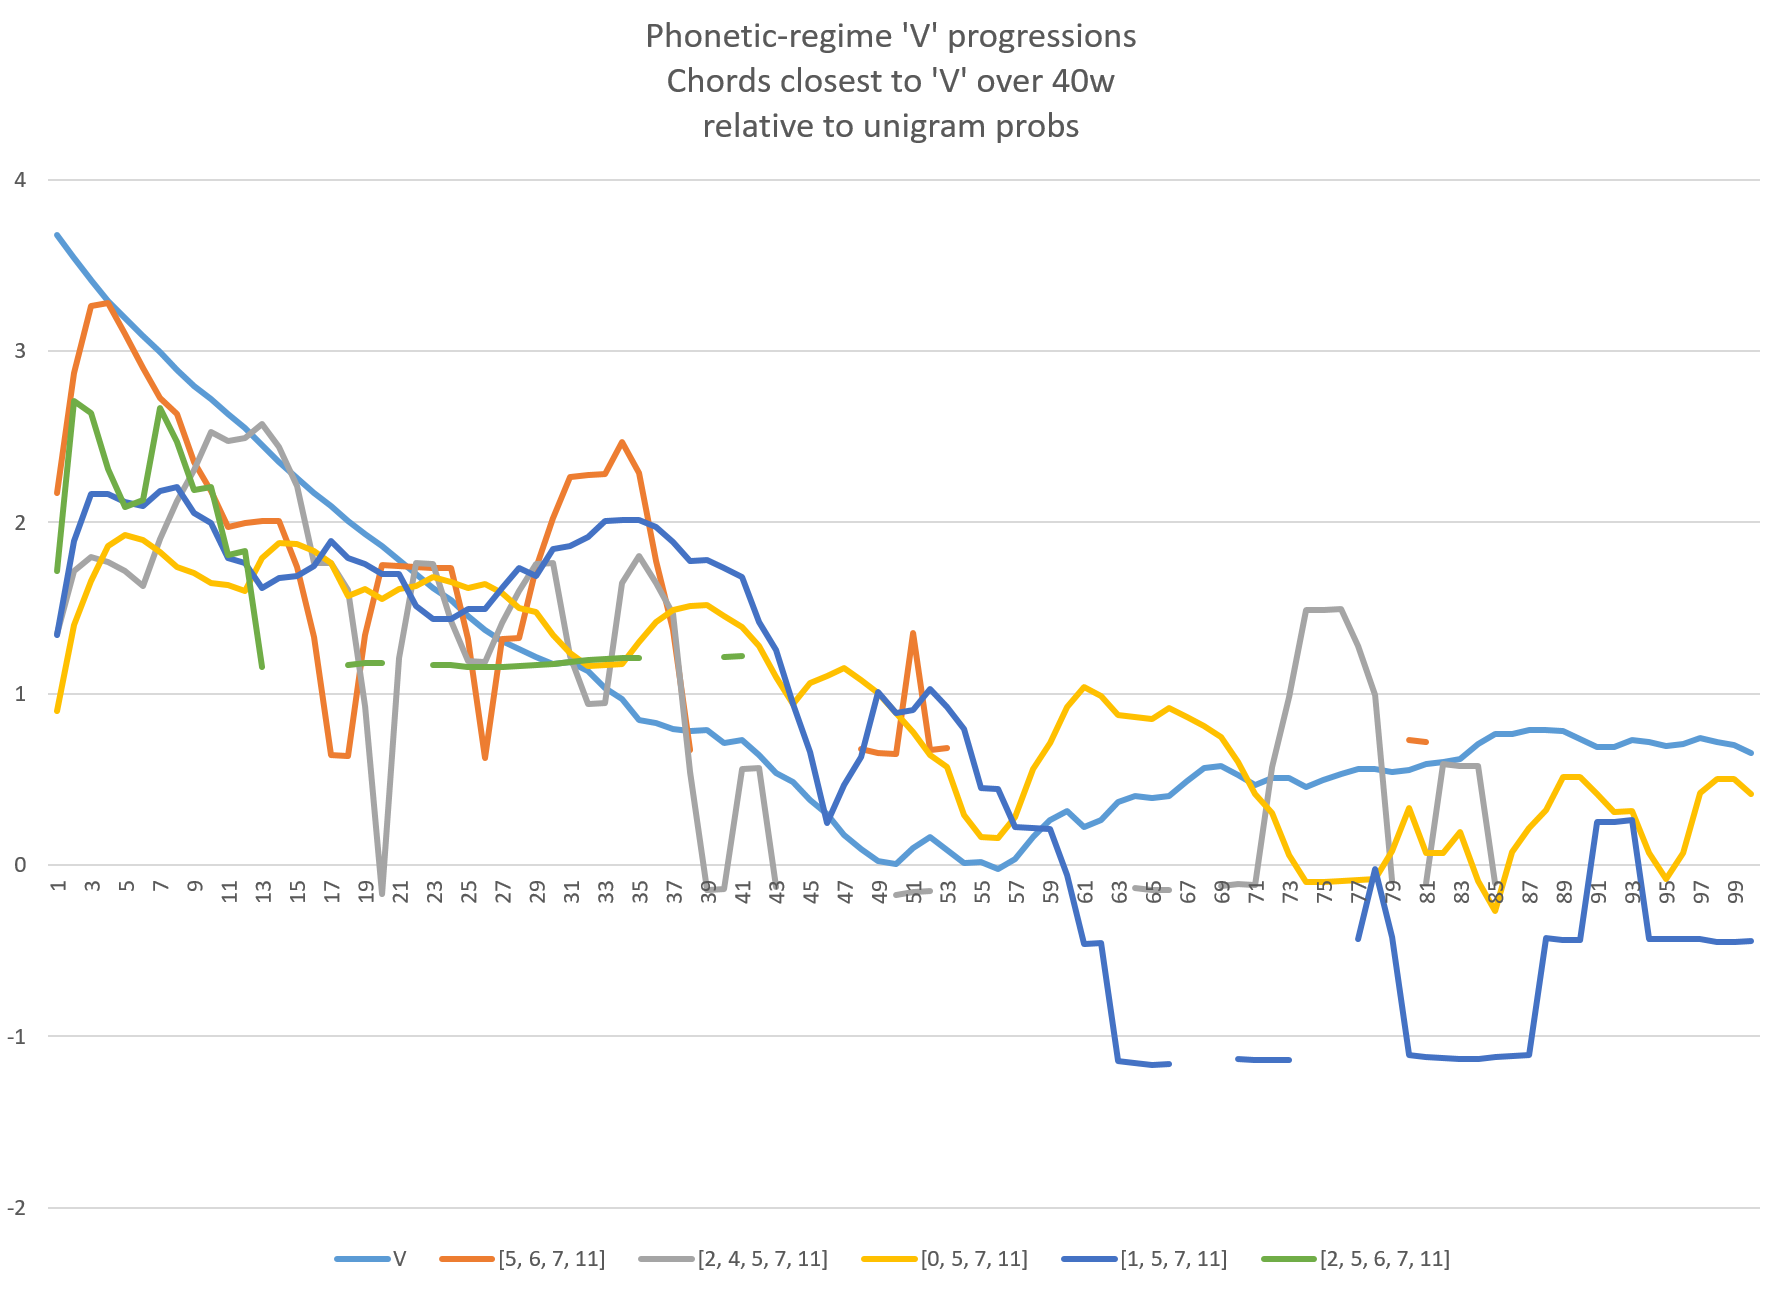
\includegraphics[width=6in]{V_phonetic.png}
\end{figure}

Syntactic regime progressions resembling $V \rightarrow I$, on the other hand, do include chords resembling $IV$, as shown in Figure~\ref{V_syntactic}.  Here, chords with temporal statistics similar to $V \rightarrow I$ cut across traditional functions and roots.  The dotted curve, $V \rightarrow [0,5,7,9]$, resembles blues progression-type motion to a $IV$ chord with an added \nth{2} or \nth{9}.  The solid curves depict ``tonic" type chords $[0,4,7,9]$ and $[0,2,3,7]$.  A human analyst might interpret the former as $I^6$ or $vi^7$, depending on its voicing, while the latter resembles a $i$ chord with added \nth{2} or \nth{9}.  But these ambiguous roman numeral assignments are unnecessary: algorithmically, these scale-degree sets participate in $V \rightarrow x$ progressions highly similar to $V \rightarrow I$, and the category of such progressions constructed here is not based on any particular chord label or root.  Figure~\ref{V_syntactic} implies other frequent progressions, as well: the red dashed curve depicts $V \rightarrow \flat III^{(M)7}$, a ``Giant Steps"-like major third progression (albeit to a major-seventh chord), while the yellow dashed curve indicates that the minor triad $[2,7,10]$ can follow $V$ in a way similar to the other destination chords plotted here.  This last progression may violate the expectations of a human analyst, indicating a site for more detailed, tune-level analysis to determine what kind of behavior is captured here.

\begin{figure}[h]
	\caption{Syntactic regime destination chords following the appearance of $V$.  Note the comparatively short time delay; $V$ does not have a strong predictive impact on the appearance of $I$ for long.  This is likely due both to the very high unigram probabilities of $I$ and $V$ and to $V$'s role in faster progressions (compared to $ii$).}
	\label{V_syntactic}
	\centering
	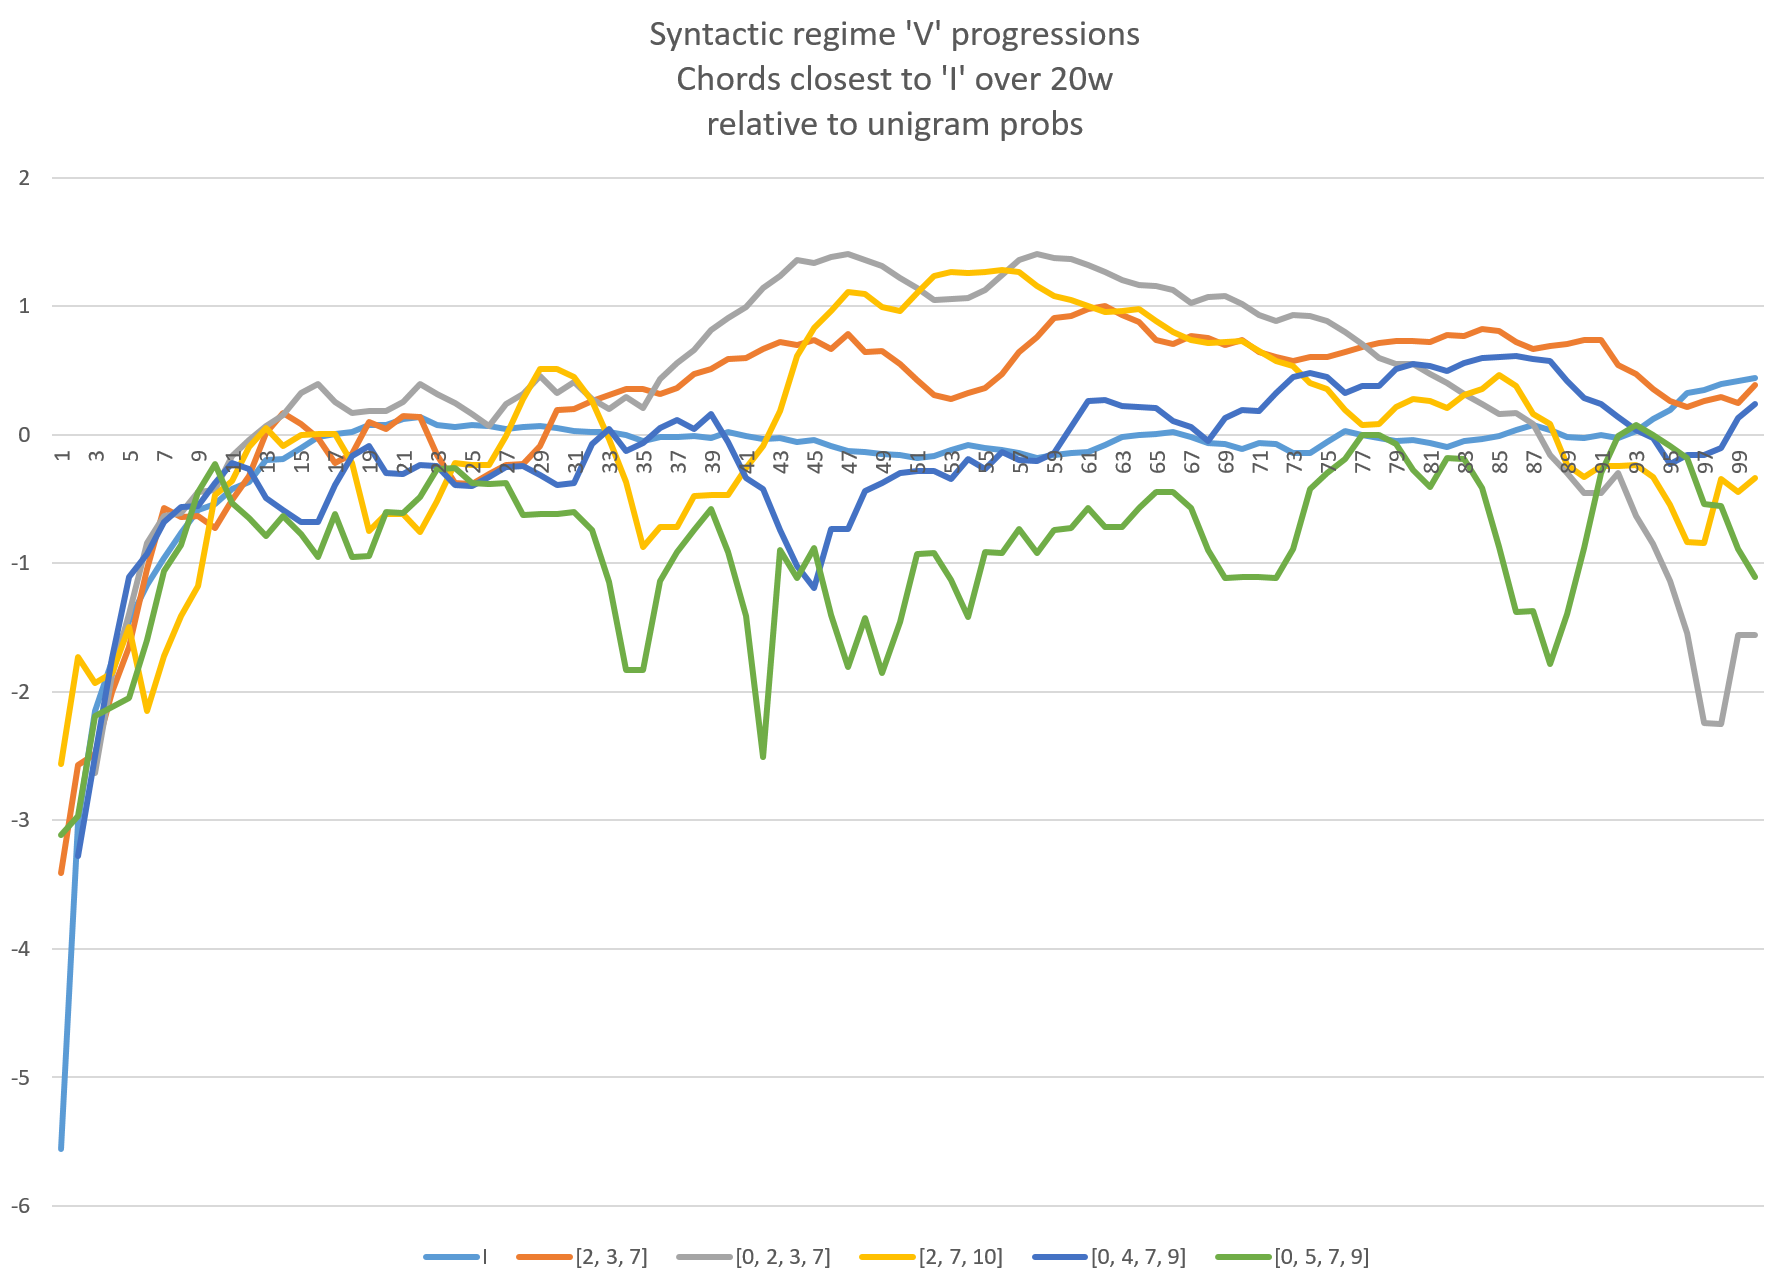
\includegraphics[width=6in]{V_syntactic.png}
\end{figure}

Approaching the phonetic and syntactic regime progressions which resemble prototypical progressions like $ii \rightarrow ii$ or $ii \rightarrow V$ for a variety of origin chords reveals a complex array of progression behaviors both expected and unexpected by a (or this) human analyst.  In these cases, interpreting a syntactic pattern from the temporal correlations between chord states involves communication between algorithmic agents and human agents with different ontological conditions for chords, keys, and progressions.  I will return to this communicative semiotics in Chapters 4 and 5.  But part of the interpretive confusion stemming from the above figures rests on their use of hand-assembled chord categories with labels like $ii,V$ and $I$.

The algorithmic agents tallying temporal statistics and extracting similar probability curves have no particular reason to identify or employ these hand-assembled categories; at the beginning of this chapter, I \emph{posited} them in order to motivate my re-description of traditional harmonic progressions in temporal terms.  But with a sense of how the temporal progression regime behavior of chords might inform syntactic category formation, Chapter 4 will use dimensional reduction and machine learning to construct new chord categories without appeals to roman numerals, root, or pitch similarity.  To enable the algorithmic agents of Chapter 4 to engage with the temporal properties of YJaMP scale degree sets, the remainder of this chapter will generalize the temporal progression regimes of the $ii$ case study above to enable their automated extraction without the necessity of \emph{a priori} intuitive prototypes.

\section{Temporal Progression Regimes}
The selection above of $ii \rightarrow ii$ and $ii \rightarrow V$ as prototypes for categories of temporal progression behavior served an important purpose.  Since probabilistic statistics connect each origin chord to a large number of destination chords, some principled method for selecting destination chords with common behaviors is necessary.  The examples used in this chapter depend on thousands of 100-dimensional vectors, each of which features its own unique shape.  Choosing temporal progression prototypes constituted a selection of shape types.  I assumed that the shapes of the $ii \rightarrow ii$ and $ii \rightarrow V$ chord distributions were common and important ones.  But the YJaMP data can suggest its own collection of shape types.

Principal component analysis (PCA) treats problems of exactly this nature in the world of time-series analysis and machine learning.\footnote{Common in the machine learning literature, PCA dates to \cite{pearson1901}.  Other machine learning techniques accomplish similar ends, and I have no proof that PCA provides optimal results -- but the structure of the time-series analytical problem here, with its presumed near-continuity between adjacent time windows, suggests the appropriateness of the tool.}  Given a data set with a high-dimensional coordinate basis -- like a set of 100-dimensional vectors -- PCA constructs a lower-dimensional coordinate system, projecting elements of the data set onto a much smaller collection of new basis vectors which best account for a maximum amount of the variance in the data.  The formal details are complex, but I offer an intuitive explanation here to connect temporal progression regimes to the PCA results.\footnote{PCA receives formal treatment in textbooks like \cite{jolliffe2002}; see especially its application to time series analysis in Chapter 12, pp.\ 299 ff.  Music theoretical projects employing PCA appear in rhythm and microtiming studies (\cite{repp1992}; \cite{benadon2015}), while the Music Information Retrieval (MIR) community applies it to extracting harmonic information and genre features from complex audio signals (see \cite{huang2014}; \cite{kaneko2010}).  My use here draws on features of both approaches.}

PCA algorithms treat a collection of observations as a sample population.  The individuals in the sample -- all the destination chords for a given origin chord like $ii$, in this case -- vary in their properties, and some are more alike than others.  After the appearance of $ii$, some destination chords will show large spikes in probability in the first few time windows compared to their corpus-wide unigram properties.  Consider how much more likely $[2,4,5,9]$ is to appear within 1.5 seconds after $ii$; Figure~\ref{ii_phonetic} indicates that it appears at this time scale almost 100 times as often as it does in the corpus at large.  But at time delays longer than about 2 seconds, $[2,4,5,9]$ displays much smaller increases in probability over its unigram statistics, crossing back and forth across 0, the value corresponding to no change from the unigram probability.  Since many phonetically-unrelated destination chords show much smaller (or nonexistent) probability spikes at this time scale, the set of all destination chords for $ii$ displays significant \emph{variance} across the first few time windows -- variance typically correlated from time window to time window, since a chord with high probability at 50ms is also likely to have a similarly-high probability at 100ms.

Conversely, at time delays beyond a few seconds, the set of destination chord probability distributions for $ii$ shows comparatively little variance, since the appearance of $ii$ has only a small impact a chord played much later.  This observation reflects the tendency on each of the log-probability plots above for destination chord probability curves to level off near zero over time.  Syntactic-regime destination chords might display yet a third kind of variance, since their probabilities might display large spikes further out in time than phonetic-regime chords and leveling off toward low-variance at later times than syntactically-unrelated chords.  The presence of many destination chords displaying these temporal behaviors will cause the overall set of all destination chords to display different patterns of temporal variance, templates capturing ways of varying in time.  PCA attempts to extract these templates by examining what combinations of time windows tend to vary together the most across the set of destination chords.  PCA ``thus can reveal whether there is more than one shared timing pattern represented in the sample," more than one way of varying over time in the presence of $ii$.\footnote{\cite{repp1992}, p.\ 240.  While Repp describes PCA in the context of expressive timing, his description of ``shared timing patterns" is still apt, here.}

Outside the temporal domain, PCA affords a geometric interpretation.  In the case of the destination chord probability distributions for $ii$, an algorithmic tallier has assigned each observation in the sample 100 coordinates, probability scores in each 50ms time window out to five seconds.  We might, with some imagination, think of each destination chord as a single point in a 100-dimensional space; the full set of $ii$'s destination chords, then, would be a cloud of such points.  Along some coordinate dimensions in that space -- like the coordinates corresponding to long times after the appearance of $ii$ -- the points of the sample cloud will be close together.  Along other dimensions, like the coordinates corresponding to very short times, the points might be quite spread out.  PCA rotates the space in which this cloud lives, identifying the ``principal axes of the ellipsoid that best approximates the cloud of data points... which coincide with the directions of maximum relative variation of the data."\footnote{\cite{benadon2015}, p.\ 25.}

The longest axis of the ellipsoid will be the direction along which the sample displays the greatest variance -- and we could imagine trivial cases where that direction is exactly aligned with one particular coordinate dimension.  If the destination chord probability distributions were identical at all time scales except for the very first time window, the direction of the first coordinate axis would account for \emph{all} of the variance in the data.  PCA could then produce a new set of coordinates which discarded 99 of the axis variables without losing any information about the differences between the distributions.  But for the actual YJaMP progression data, the distributions usually vary over all 100 time scales, many of which are non-trivially correlated.  It might be that chords in the phonetic regime primarily vary over 20 windows, and that the variance in each of those windows is strongly correlated.  If those variances are similar, a PCA algorithm will select as a basis vector -- a direction of the ellipsoid approximating the cloud of points -- some linear combination of the original axes that is maximally aligned with the direction of greatest variance.

After identifying the new axis along which the variance is greatest, the first ``principal component," PCA repeats the process to identify the other highest-variance axes such that the resulting coordinates are still independent and orthogonal.  Each further principal component calculated will capture a smaller share of the overall variance in the population, and an analyst can choose the point of diminishing returns: if 20 coordinates capture 99\% of the variance between 100-dimensional observations (like our destination chord probability distributions), the analyst has little reason to introduce the complexity of an additional 80 coordinates.  This optimized reduction in coordinate complexity is one primary benefit of PCA; the production of template-like principal components is another.

For our case, the principal components can provide automated, data-driven indications as to what different kinds of temporal progression regime there might be, and they present shape types indicative of the types of variance to expect.  Running PCA on the large number of destination chord probability distributions for $ii \rightarrow x$ decomposes the high-dimensional time-based coordinates into a low-dimensional basis of temporal progression regimes.\footnote{Many commercially available standalone software packages offer PCA support.  The implementation I employ in Python comes from the package scikit-learn.  See \cite{scikit-learn}.}  Figure~\ref{ii_pca} plots the first 5 machine-generated principal components for $ii$ chord destinations.

\begin{figure}
	\centering
	\caption{The top 5 principal components calculated from the full set of destination chord temporal probability distributions following $ii$.  The plot is of probability versus time; the legend indicates the components and their variance percentages in descending order.}
	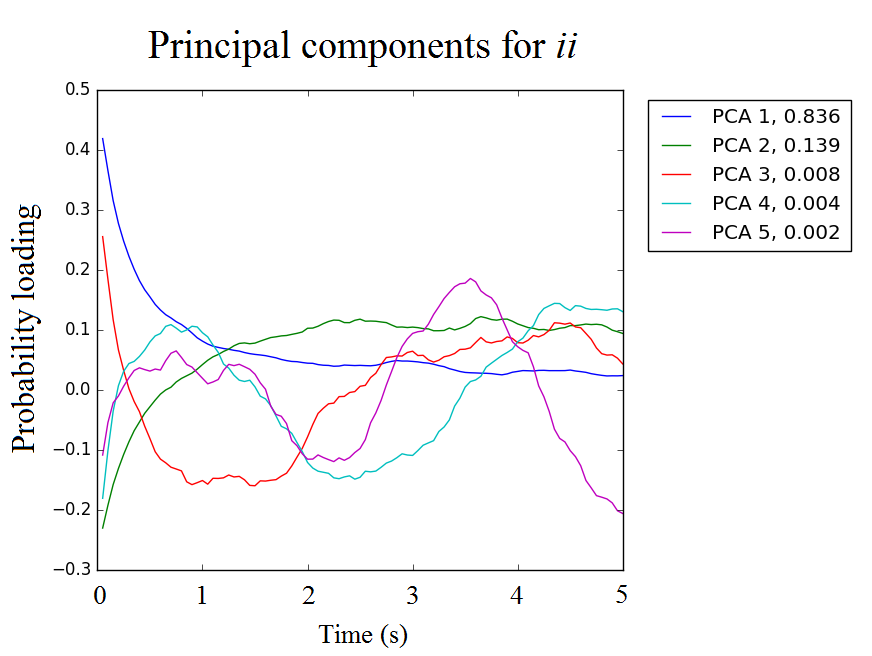
\includegraphics[width=6in]{iipca_ABS_ed.png}
	\label{ii_pca}
\end{figure}

With slight theoretical adjustments, I propose that these distribution shape classes (or, more properly, combinations thereof) can be used in place of the hand-picked $ii$, $V$, and $I$ shape templates employed earlier in the chapter for the assembly of phonetic and syntactic progression regimes.  The first principal component, the blue curve on the figure, accounts for most of the variance in the distributions; large positive and negative scores with respect to this component indicate behavior where the shorter time spans vary much more than the longer ones, which approach their unigram probabilities.  This behavior is comparable to that of the phonetic regime.  Component 2, the green curve, captures chords with large initial variance, but which level off at a non-zero log probability relative to their unigram statistics.  Chords with large positive coordinates along this component are initially suppressed but predicted later, much like non-phonetic chords that do have tonal relevance to phrases in which $ii$ appears (compare this to $ii \rightarrow I$ on Figure~\ref{iiprog}).  Components 3-5 indicate more nuanced variance behavior, though they only account for a very small percentage of the data's variance: as indicated by the legend, the lion's share of information is captured by the first two components.  Component 3, for example, resembles the exact opposite of the $ii \rightarrow V$ syntactic regime prototype.  Multiplying this component by negative one yields a template which starts with phonetic-regime probability suppression, rises to a probability peak between 1 and 2 seconds, and then falls toward the unigram probability. 

To a human analyst, these machine-generated regimes of chord behavior might seem to provide a framework subsuming both ``embellishing" and ``harmonic" progressions -- a general statistical basis for temporal progression behavior.  They rely on no particular knowledge regarding the pitch content of the chords involved, and they suggest a crude binary: that the kinds of chords traditionally reduced away as voice-leading neighbors or functional prolongations might be those which most resemble PCA component 1, while chords identified as part of syntactic progressions might score low along component one and higher along some other appropriately shaped component.

In some cases, this may be true, but it offers no proof or disproof of traditional reduction techniques.  As Chapter 4 will indicate, interpreting these components in isolation requires caution, since destination chords can be described by positive and negative multiples of each component as well as combinations of more than one.  For any given origin chord, the relationship between its principal components and reduction or progression expectations may be less clear than for the $ii$ case study presented here.  With this in mind, the immediate interpretive payoff of the components for a human analyst, though suggestive, is comparatively small.

But I will argue that the algorithmic payoff for a pipeline producing syntactic categories is large: describing an origin chord in terms of the most common ways its destination chords progress in time allows algorithmic agents to use temporal progression statistics as the basis for chord category formation.  Moreover, it does so in a way free of the bigram-like state-to-state transitions assumed in score-based, roman numeral adjacency models of harmonic syntax.  In a sense, time series analytical PCA allows the algorithmic agents to take advantage of much more information than would be encoded in merely adjacent progressions.  Generalizing across temporal regimes widens the scope of harmonic progression inquiry without invoking recursive grammars, Schenkerian prolongations, or pre-determined surface reduction rules.